\chapter{Design and Implementation}

\begin{figure}[here]
\center
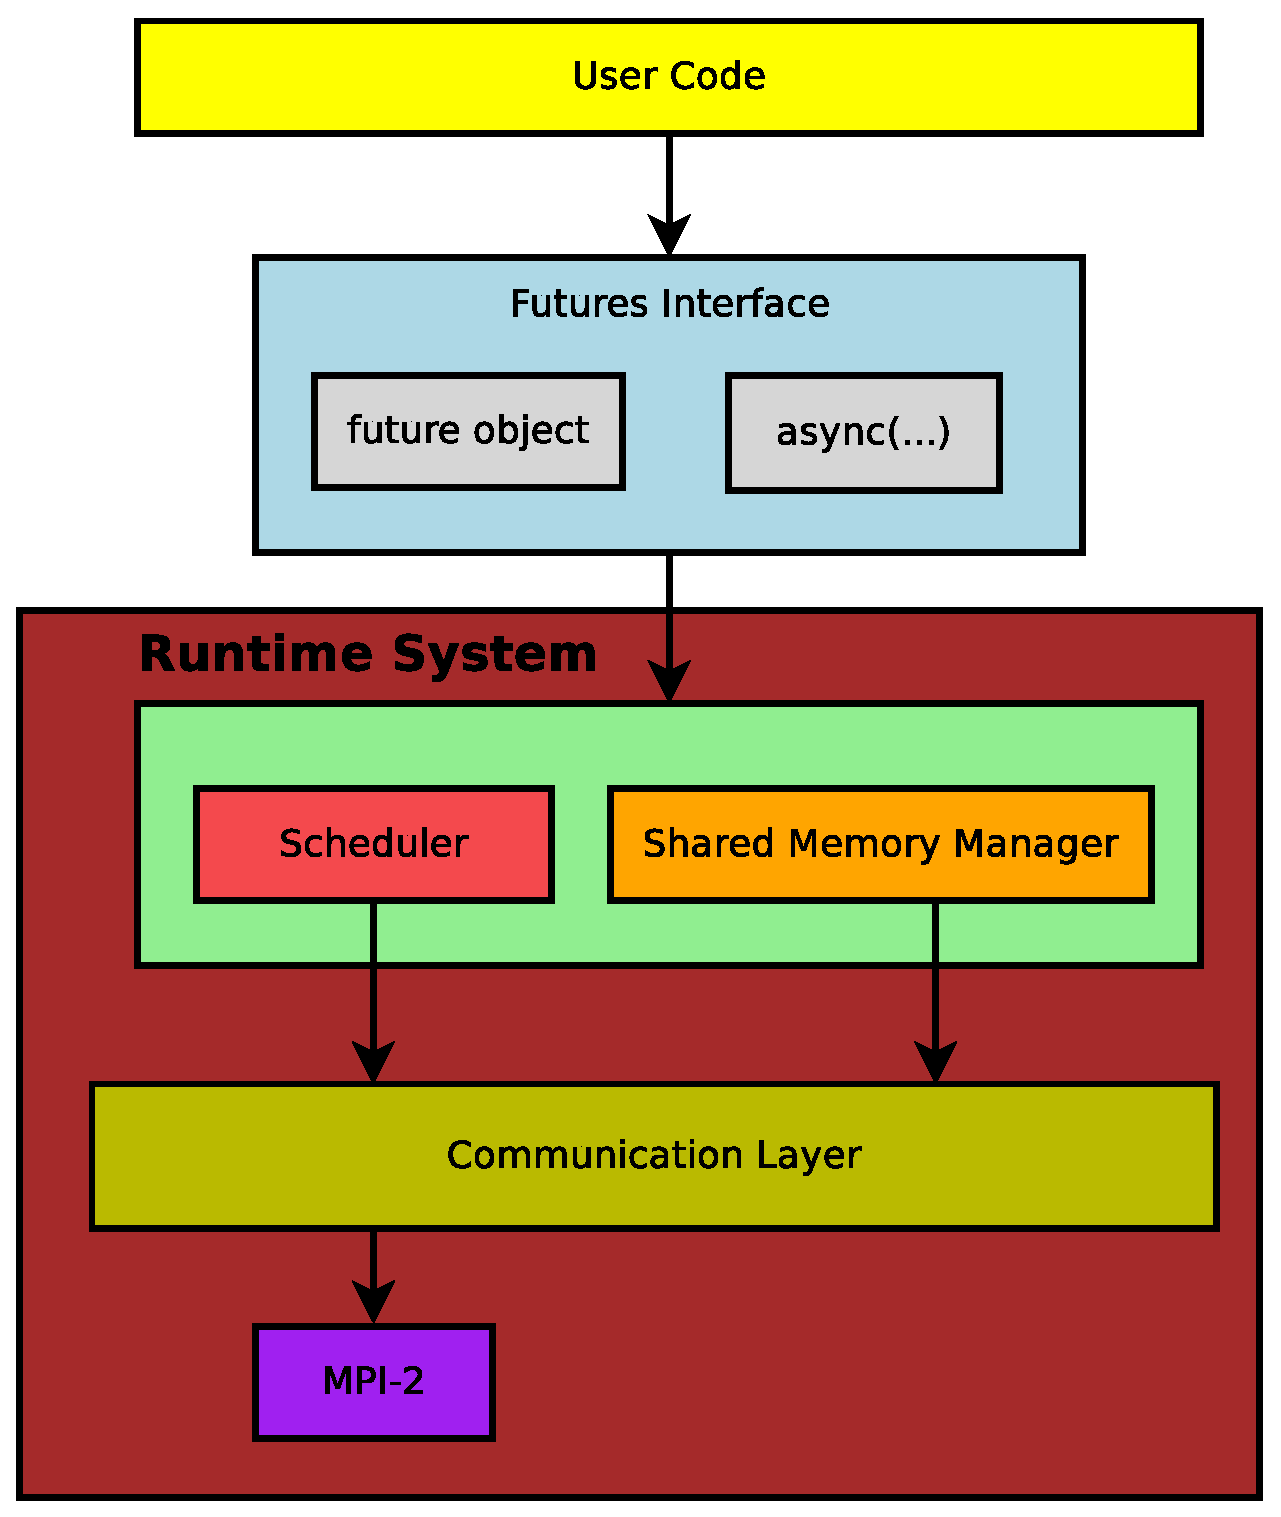
\includegraphics[width=0.7\columnwidth]{figures/system_overview}
\caption{Overview of our futures library design.}
\label{fig:system_overview}
\end{figure}

We have modeled the distributed futures, as closely as possible, 
to the shared memory futures from the C++ standard library.  Parallelism in the future
model is extracted by issuing functions asynchronously, using a \emph{special} async funtion
that takes the function to be executed in parallel as an argument (see section ~\ref{sect:futures-interface}).
In our library, functions called using the async function,
refered to as \emph{jobs} from now on, are send through a communication library 
to be executed by other avaible processes.  
The decision of who executes a \emph{job} is made by a scheduler.  The host process can retrieve
the return value of a \emph{job} using the future object associated with the corresponding \emph{async} call.
A process can only retrieve a future's value if the job has finished executionm, in which case the remote 
process will set the futures value on the host process, else the host process will will block.
In our implementation, a blocked process will try to execute any pending \emph{jobs} it might have
while it is beeing blocked.
		We designed our system so that different aspects of the runtime library, such as process
communication, hide its underlying implementation (e.g. MPI),  thus different implementations 
of the same module should not interfere with other components of the library.
Figure~\ref{fig:system_overview} shows the different component hierarchy.\\
\\
Our system consists out of three main modules:
\begin{itemize}
	\item The \textbf{communication} module, which is the backbone of the system
	and used by all other components in order to exchange messages and create a shared address space.

	\item The \textbf{Shared Memory Manager}, which is an allocator for the shared address space between the processes.

	\item The \textbf{Scheduler}, which is responsible of handling how \emph{jobs} are send/received between processes
	and also decides which process will run a \emph{job}.
\end{itemize}

\vfill

All the above modules are initialized, finalized and managed by an system environment, 
an instance of which is present
at every process.  Note that it is not necessary however for every environment instance to be the same, for
example process 1 can be only responsibe for it's own shared address space and be aware only of the shared
addresses of other processes, which hold futures associated with \emph{jobs} that are supposed to run by
process 0.

\begin{figure}[here]
\begin{lstlisting}
class helloWorld {
public:
	helloWorld() {};
	~helloWorld() {};
	int operator()() { 
		int id = Futures_Id();
		cout << "- Worker" << id << ":Hello Master" << endl;
		return id;
	};
};

FUTURES_SERIALIZE_CLASS(helloWorld);
FUTURES_EXPORT_FUNCTOR((async_function<helloWorld>));

int main(int argc, char* argv[]) {
	Futures_Initialize(argc, argv);
	helloWorld f;
	future<int> message = async(f);

	cout << "- Master :Hello " << message.get() << endl;

	Futures_Finalize();
};
\end{lstlisting}
\caption{
A simple hello world implementation using the distributed futures interface.  
The output of the program on process 0 would be "- Master :Hello 1".}
\label{lst:hello}
\end{figure}

\begin{figure}[here]
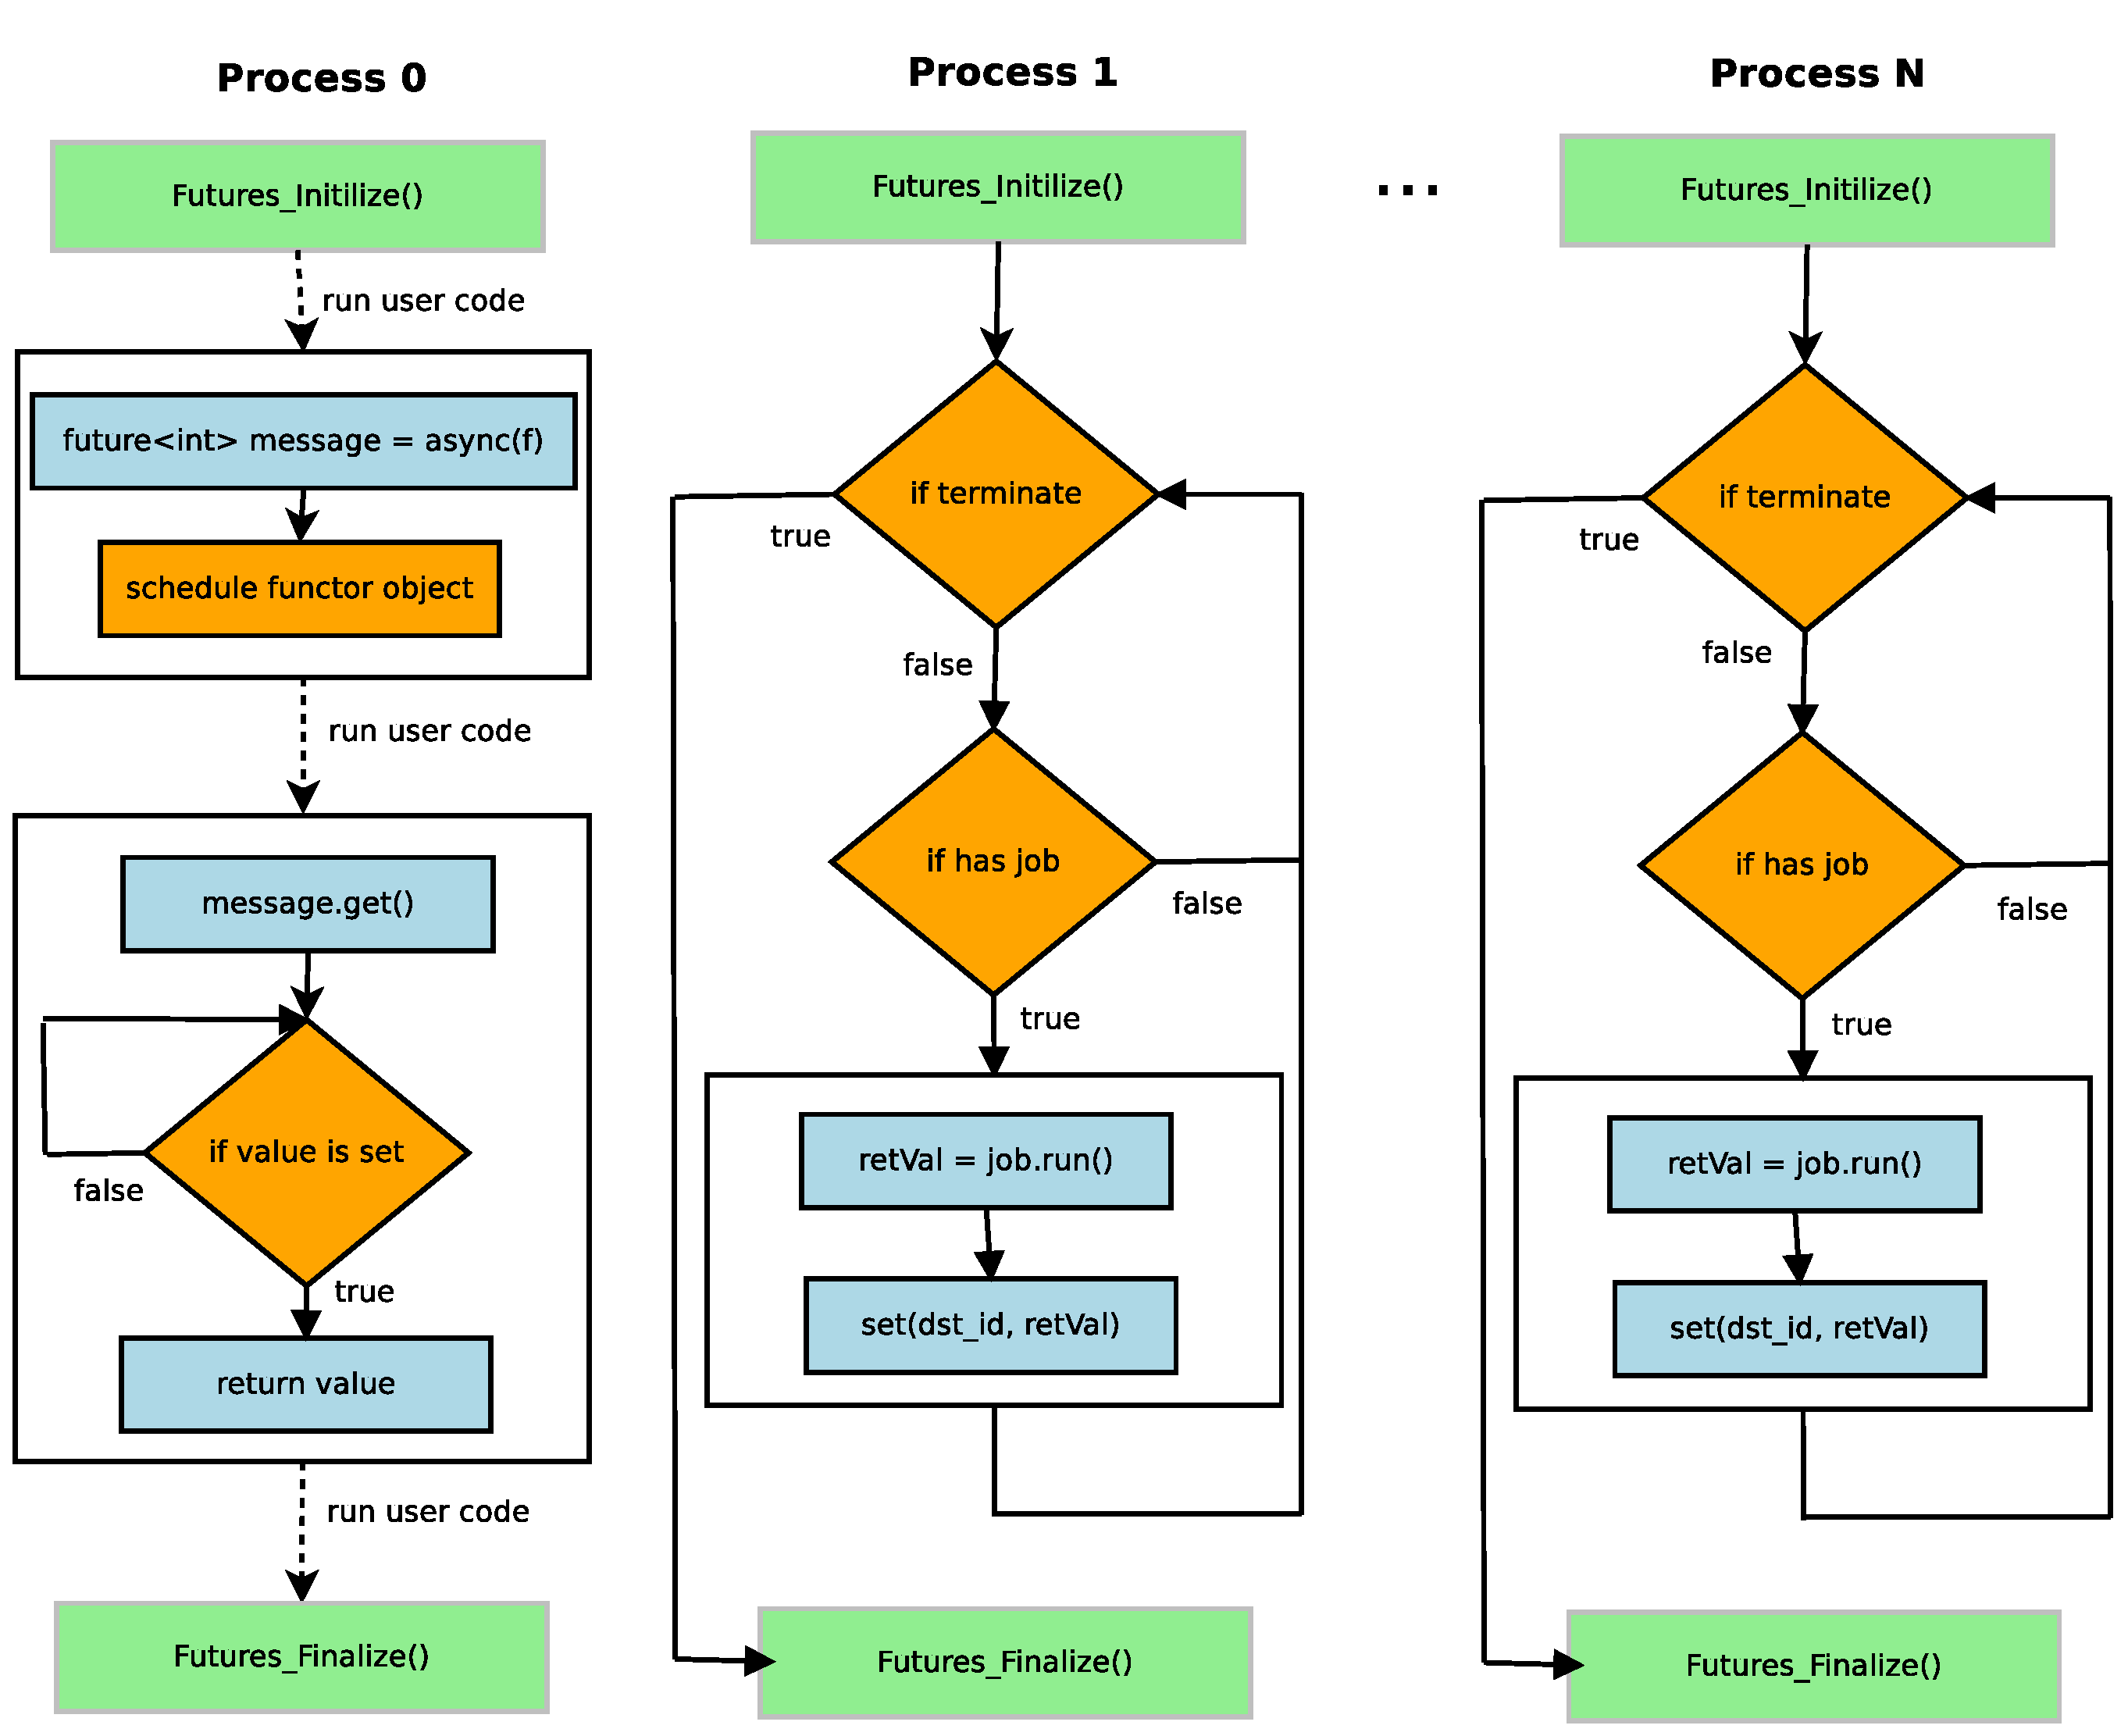
\includegraphics[width=\columnwidth]{figures/hello_flow}
\caption{
The control flow of the hello world program in figture~\ref{lst:hello}.}
\label{fig:helloCF}
\end{figure}

Figure~\ref{fig:helloCF} shows the program flow for processes 0 and 1, of the simple
hello world example in figure~\ref{lst:hello}.  Before any call to the library is made, the futures
environment must be initialized, which in turn initializes all other library modules 
(e.g. communication, scheduler, memory manager).
All processes execute the main function, but only
the master process will return from it and continue with the user program execution.
All other processes will run our runtime's scheduler code and wait to receive \emph{jobs}.
The \emph{async} function can be called from any process 
and within other async calls, thus allowing recursive algorithms to be expressed. 
In the example, process 0 issues a \emph{job} by
calling \emph{async(f)}.  It will then return from the call and continue until
the message.get() call, at this point the process will either retrive the message value or block untill
it's set.
The job is then scheduled to be executed by process 1.  The worker process,
here process 1, will wait until a \emph{job} is send and then run it.  When done, it will set 
the future's value and return to waiting for other jobs or until it is terminated by the master
process.  When process 0 retrieves message's value, it prints it and continues until it reaches
the Futures\_Finalize() routine.  At this point it will singal all other processes that the program
has reached it's termination point and finalize the futures environment.  All other processes will
do the same after receiving the terminate signal.
\\

In the rest of this chapter, we will present the future interface in section~\ref{sect:futures-interface}
and discuss our implementations of the the communication, shared memory manager and scheduler modules in
sections~\ref{sect:communication},~\ref{sect:shared-memory-manager} and~\ref{sect:scheduler}
respectively.

\section{Futures Interface}
\label{sect:futures-interface}
We replicate the futures interface from the C++ standard threads library, with one major difference being that 
the the function being called must be a functor object.  Figure~\ref{lst:fib} shows a recursive implementation
of the fibonacci function using our future implementation.  The user needs to create a functor, which must be
serializable, and use the macro 
FUTURES\_EXPORT\_FUNCTOR(async\_function<fib, int>) to expose the functor object to the underlying 
serialization library \footnote{We use the boost serialization library~\cite{Ramey:2004:Boost:Serialization} 
and the input/output archives from the boost mpi library~\cite{Gregor:2005:Boost:MPI}}.
Moreover, the user can use the FUTURES\_SERIALIZE(F) macro, where F is a functor object, 
which will create the necessary serialization routines automatically, but it is not recommended if the 
functor object has members (see~\cite{Ramey:2004:Boost:Serialization} for more details on how to serialize
a C++ object with Boost serialization library).
Note that the argument to the first macro command is always \emph{async\_function<F, Args...>},
where F is a functor class
and Args are an aribary number argument types, that are to be passed to the overloaded call method 
of the functor F.  \emph{Async\_function} is a special class that wraps around the functor objects and its
arguments.  Instantiation of this class, using C++ templates metaprogramming capabilities,
generates the appropriate routines, for setting the future's value, according to the value's type.
It also facilitates all necessary information that are needed to be transfared to the worker process.
Figure ~\ref{lst:async_function} shows the definition of the \emph{async\_function} class.


A call to the \emph{async(F, Args...)} function, where F is a functor object and Args 
is any number of arguments,
will send the functor object to an available process or execute 
the functor directly, if no such process is found (see~\ref{sect:scheduler} for details). 
The async function returns a 
future object which can be used by the process that called the \emph{async} function to retrieve the 
functor's return value.  If the return value is an array, a pointer or any other form of container, the user
should instead call a variation of the \emph{async} function, \emph{async(N, F, Args...)}, 
where N is number of elements that will be returned. In order to retrieve the value,
the owner of the future needs to call the get() method.  This method is blocking, so calling it will cause the 
process to block until the value of the future becomes available.  Alternatively, the future owner can call the
is\_ready() method, which is not blocking, to check if the value can be retrieved, and if not continue running
user code until the future's value becomes available at a later point.  Also, note that before using
the futures library, the user has to explicitely call the \emph{Futures\_Initialize()} and \emph{Futures\_Finalize()},
which will initialize and finalize the futures environment, respectively. 

\begin{figure}[here]
\begin{lstlisting}

template<typename F, typename... Args>
class async_function : public _job {
... //we have ommited here all the serialization routines
public:
		int src_id;
		int dst_id;
		Shared_pointer ptr;
		int data_size;
		int type_size;
    F f;
  	std::tuple<Args...> args;
    typename std::result_of<F(Args...)>::type retVal;
    async_function();
    async_function(int _src_id, int _dst_id, 
									Shared_pointer _ptr, 
									int _data_size, int _type_size,
									F& _f, Args... _args);
    ~async_function();
    void run();
};
\end{lstlisting}
\caption{The \emph{async\_function} function class definition.  All \emph{jobs} in our system are
instances of this class.  The base class \emph{\_job} is used for serialization purposes as well.}
\label{lst:async_function}
\end{figure}

\begin{figure}[here]
\begin{lstlisting}
class fib {
public:
	fib() {};
	~fib() {};
	int	operator()(int n) {
		if(n == 0) return 0;
		if(n == 1) return 1;
		fib f;
		future<int> fib1 = async(f, n-1);
		future<int> fib2 = async(f, n-2);
		return fib1.get() + fib2.get();;
	};
};

FUTURES_SERIALIZE_CLASS(fib);
FUTURES_EXPORT_FUNCTOR((async_function<fib, int>));

\end{lstlisting}
\caption{A fibonacci implementation using the distributed futures interface}
\label{lst:fib}
\end{figure}



\section{Communication}
\label{sect:communication}
The communication module is responsible for message exchange between all of the processes in our system,
as well as providing the infrastructure for a shared address space.
In our implementation the communication module uses MPI-2'S one-sided communication libary and Boost MPI's
input and output archives, for object serialization.

The communication module acts as a layer of abstraction between the various system component and the MPI libary.
It acts as a simple wrapper for initializing, finalizing MPI and simple send/receive operations.
It is also capable of providing information of the MPI environment to the other components of our system (e.g.
number of processs, rank e.t.c.).  Moreover, it can be used to expose part of a process' address space to other 
processes in the same commuication group.  

\subsection{Shared Address Space}
In our implementation, the underlying message passing library used is MPI-2, thus we use MPI windows to
expose such space among processes.  
Exposing part of process' address space in the MPI-2 schema, requires that the some
space will be locally allocated to a pointer using the MPI\_Alloc\_mem, and then exposed to other processes
through creating an MPI window that is correlated to the pointer with MPI\_Create\_Win 
(See section~\ref{sect:mpi-one-sided}). 
A drawback in MPI is that a window can be created only collectively over an MPI communicator,
and in turn, a communicator can be created, again, only collectively over an existing paretnt communicator. 
In our design, this requires that either all windows are created a priori at initialization, 
since when issuing a job, only the sender and receiver should take part in the communication.  
In order to overcome this limitation, we implemented the algorithm presented in
~\cite{Dinan:2011:NCC:2042476.2042508}, which requires only the processes that will join the communicator to
take part in the communicator creation process.  The algorithm needs an MPI group as input and progressively
creates two adjacent groups of processes.  If a process' id is even, then the process is added to the \emph{right}
group, if the process' id is odd it is added to the \emph{left}.  Everytime a process is added to either group, an
inteprocess communicator is created and then merged with the adjacent group's interprocess communicator. The 
algorithm's pseudocode can be found on~\cite[p.287~]{Dinan:2011:NCC:2042476.2042508}.
Employing this algorithm we can dynamically allocate windows between any two processes that compose an MPI group.

\begin{figure}[here]
\begin{lstlisting}
void set_data(void* val, int dst_id, Shared_pointer ptr, 
							Datatype datatype) {

    MPI_Win_lock(MPI_LOCK_EXCLUSIVE, dst_id, 0, 
								shared_space[ptr.page_size]);

    MPI_Put(val, ptr.size, datatype, dst_id, ptr.base_address, 
						ptr.size,	datatype, shared_space[ptr.page_size]);

    MPI_Win_unlock(dst_id, shared_space[ptr.page_size]);
};

void set_data(boost::mpi::packed_oarchive& ar, int dst_id, 
							Shared_pointer ptr) {

    MPI_Win_lock(MPI_LOCK_EXCLUSIVE, dst_id, 0, 
								shared_space[ptr.page_size]);

    MPI_Put(&ar.size(), 1, MPI_INT, dst_id, ptr.base_address,
						1, MPI_INT, shared_space[ptr.page_size]);

    MPI_Put(ar.address(), ar.size(), MPI_PACKED, dst_id, 
						ptr.base_address+DATA_OFFSET,
						ar.size(), MPI_PACKED, shared_space[ptr.page_size]);

    MPI_Win_unlock(dst_id, shared_space[ptr.page_size]);
};
\end{lstlisting}
\caption{The function used to set a future's value.  The first version is for primitive data types, 
where as the second is for serializable objects.}
\label{lst:set_data}
\end{figure}

The communication library also provides the routines needed to write and read data from a address space shared
though an MPI window, using the special Shared\_pointer construct (see section~\ref{sect:shared-memory-manager}).  
This pointer keeps information of where the data is located within an MPI window in addition to the total size of the data associated with this pointer during its allocation.  Figure~\ref{lst:set_data} shows a simplified version for 
setting a future's value.  The ptr variable has information on the location we need to write the data to on an MPI 
window.  The shared\_space[ptr.page\_size] is a map that contains mpi windows.  Section
~\ref{sect:shared_memory_manager} explains how MPI windows are organized in this map, according to the 
page sized used during allocating space for a future.  Note that the variable datatype, MPI\_Datatype in this
implementation, is inferred statically using template routines from the Boost MPI libarary,
when instantiating the \emph{async\_function} class.  The second overloaded \emph{set\_data} method is used for
when the future's value is not a primitive data type and requires serialization.  In the latter scenario, we
need to store information on the archives size, thus the actual data is indexed at location 
ptr.base\_address+DATA\_OFFSET.

\subsection{Mutexes}
In order to synchronize accesses to shared memory addresses and other critical sections in our system, designed
a mutex library, whith the same interface as the standard C++ mutex library, which is implemented
for shared memory.  The only difference is that a call to lock, unlock or try\_lock requires the user to specify
the id of the tareget process. We have adopted MPICH's implementation of mutexes in our design.  A mutex is a
shared vector through an MPI window.  Each vector element is a byte value corresponding to one process.  When
a process wants to hold the mutex lock, it sets its vector value at one and iterates through the rest of the 
vetor to check if another process wants or has acquired the lock.  If the lock is acquired or another process 
waits for it, then the current process blocks until it receives a message.  When unlocking, a process sets its 
vector value to zero and then iterates through the vector to find and send a message to next process that is 
waiting to acquire the lock.  

\section{Shared Memory Management}
\label{sect:shared-memory-manager}
The Memory Manager module is responsible for managing the systems shared address space. 
It uses the communication module to create address spaces that
are visible by all processes in our system and use the Shared\_pointer construct to describe a location in such
shared memory.  This modules provides the functionallity of allocating and freeing space, from the shared address 
space among all processes.  Our allocator is implemented using free lists in order to track free space as 
described in~\cite[p.~185-187]{Tanenbaum:2007:MOS:1410217}.  
However, we keep different free lists for different page sizes to deal
with memory segmentation. Figure~\ref{fig:freeLists} shows how the memory manager keeps a map of free lists
indexed by a memory page size.
The shared address space is allocated a priori
using the communication module, to create MPI windows in our current implementation.  This is ofcourse transparent to
the Shared Memory Manager module, since it uses Shared\_pointers to describe memory location, size etc.  
The Shared\_pointer is a tuple  ptr<ID, BA, SZ, PSZ, PN, ASZ>, where id is the id of the process
whose address space we want to address, BA is the base address that the data is located in a shared address space,
SZ is the size of the data we want to allocate, PSZ is the page size the allocator used to allocate for this data,
PN is the number of pages used and ASZ is the the actual size, which is PN*PSZ.  The information tracked by a 
Shared\_pointer can be effectively used by the communication module to read/write data.  The Shared Memory Manager
modules simply holds a mapping of the shared address space, the actual local addresses are handled by the 
underlying communication library (MPI in our case).   
So, each freeList in figure~\ref{fig:freeLists} is actually a list of 
Shared\_pointers to a corresponding MPI window.  We choose
to keep seperate windows for each free list because when acquiring an epoch access to an MPI window, the whole 
window is locked, so even though we do not have overlapping accesses \footnote{only one process needs to write to a 
future's shared address, since only one future is associated with one \emph{job}.} 
(see section~\ref{sect:mpi-one-sided}).  

\begin{figure}[here]
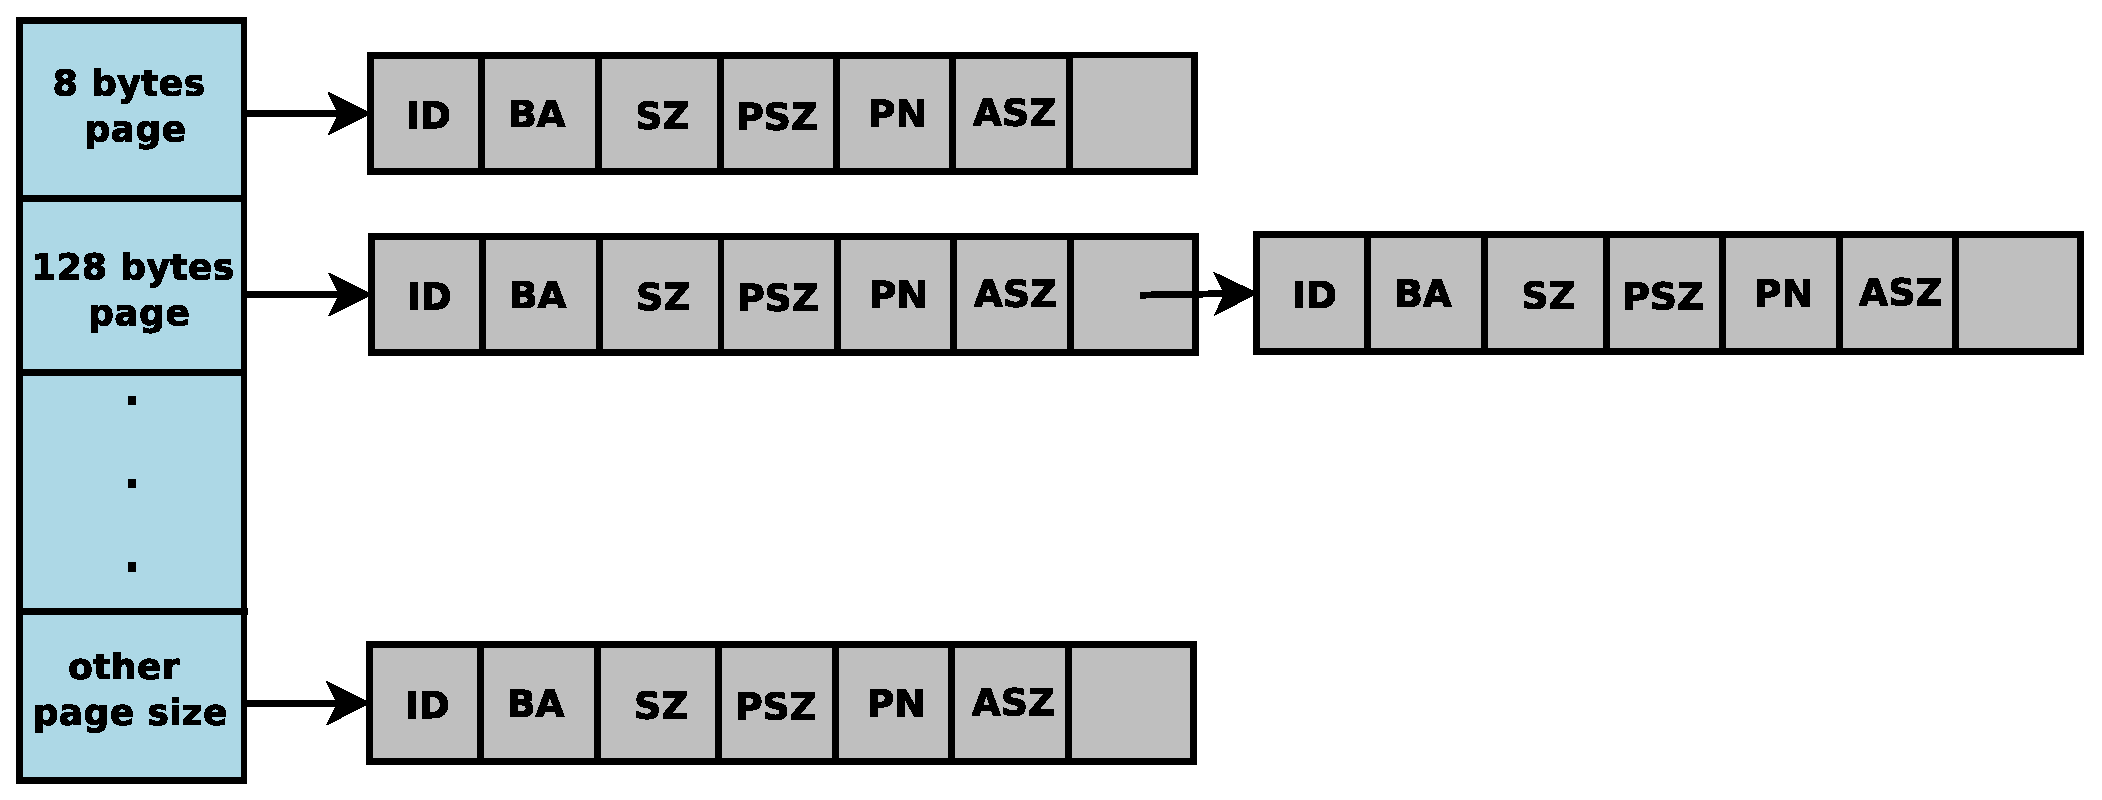
\includegraphics[width=\columnwidth]{figures/free_lists}
\caption{Shared Memory Manager keeps a map of free lists, indexed by the page size.  For page size that do
not match any predefined ones, we use the \emph{other} page size free list.}
\label{fig:freeLists}
\end{figure}

\subsection{Memory Allocation/Deallocation}
When a process issues an \emph{async} function, it needs to allocate space in its shared address space, for the worker process to store the future's value.  To allocate such space, the host process uses the shared memory manager. 
The shared memory allocator tries to find the best page size
fit for the data size, and searches the corresponding free list, using a first fit algorithm to find a large 
enough space for the new data. If no fitting page size is found then the allocator uses a special freeList, 
which does not use a predefined page size, but instead uses the data size to find free space.  If not enough free
space is found in the correct free list, then the allocator can try to find data in another free list, of different
page size.  Figure~\ref{fig:alloc} shows a free list, before and after allocating a data object.
The first fit algorithm
will iterate the list from the start untill it finds a large enough space for the object.  Each node in the free list,
is a Shared\_pointer, which describes how much continueous space there is avaible.  When the allocator finds a large
enough node, it removes from that node the size and number of pages it needs and sets its base address value 
accoringly.
It then returns a new Shared\_pointer, that describes the memory space that will be now occupied from the data object.
In the example in figure~\ref{fig:alloc}, the first list node has enough space to fit an 128 size data object.  
Removing the reserved now space, from the beginning of the list, will leave us again with two free nodes, but the
first one will now have 512 bytes left and the base address will be moved at the 128th byte.

\begin{figure}[here]
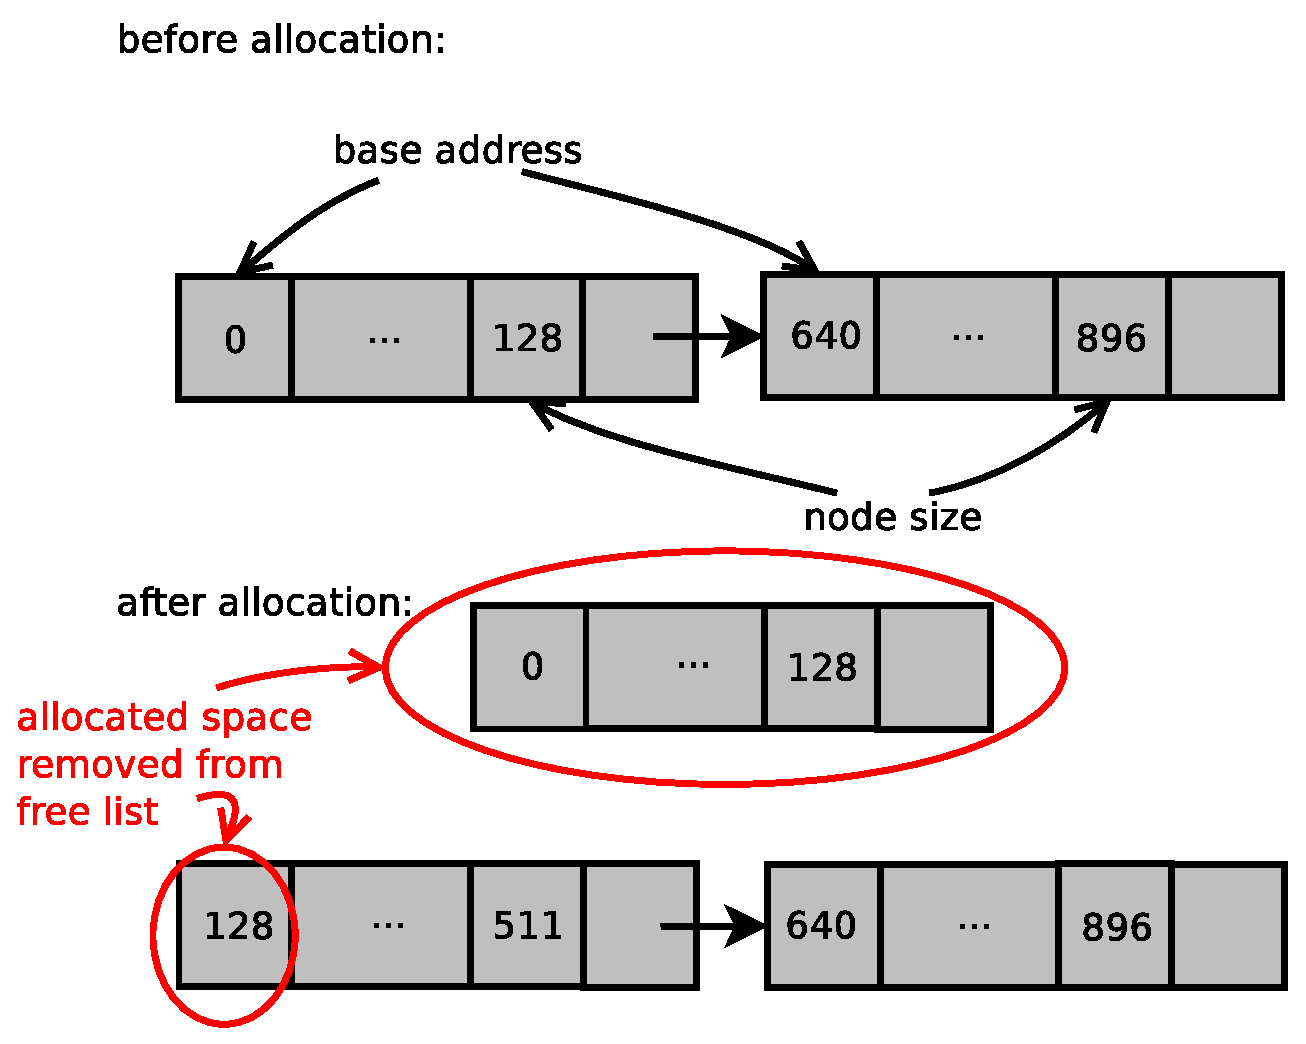
\includegraphics[width=0.6\columnwidth]{figures/alloc}
\caption{During allocation, when a large enough space is found, the allocated page is removed from the node.}
\label{fig:alloc}
\end{figure}

\begin{figure}[here]
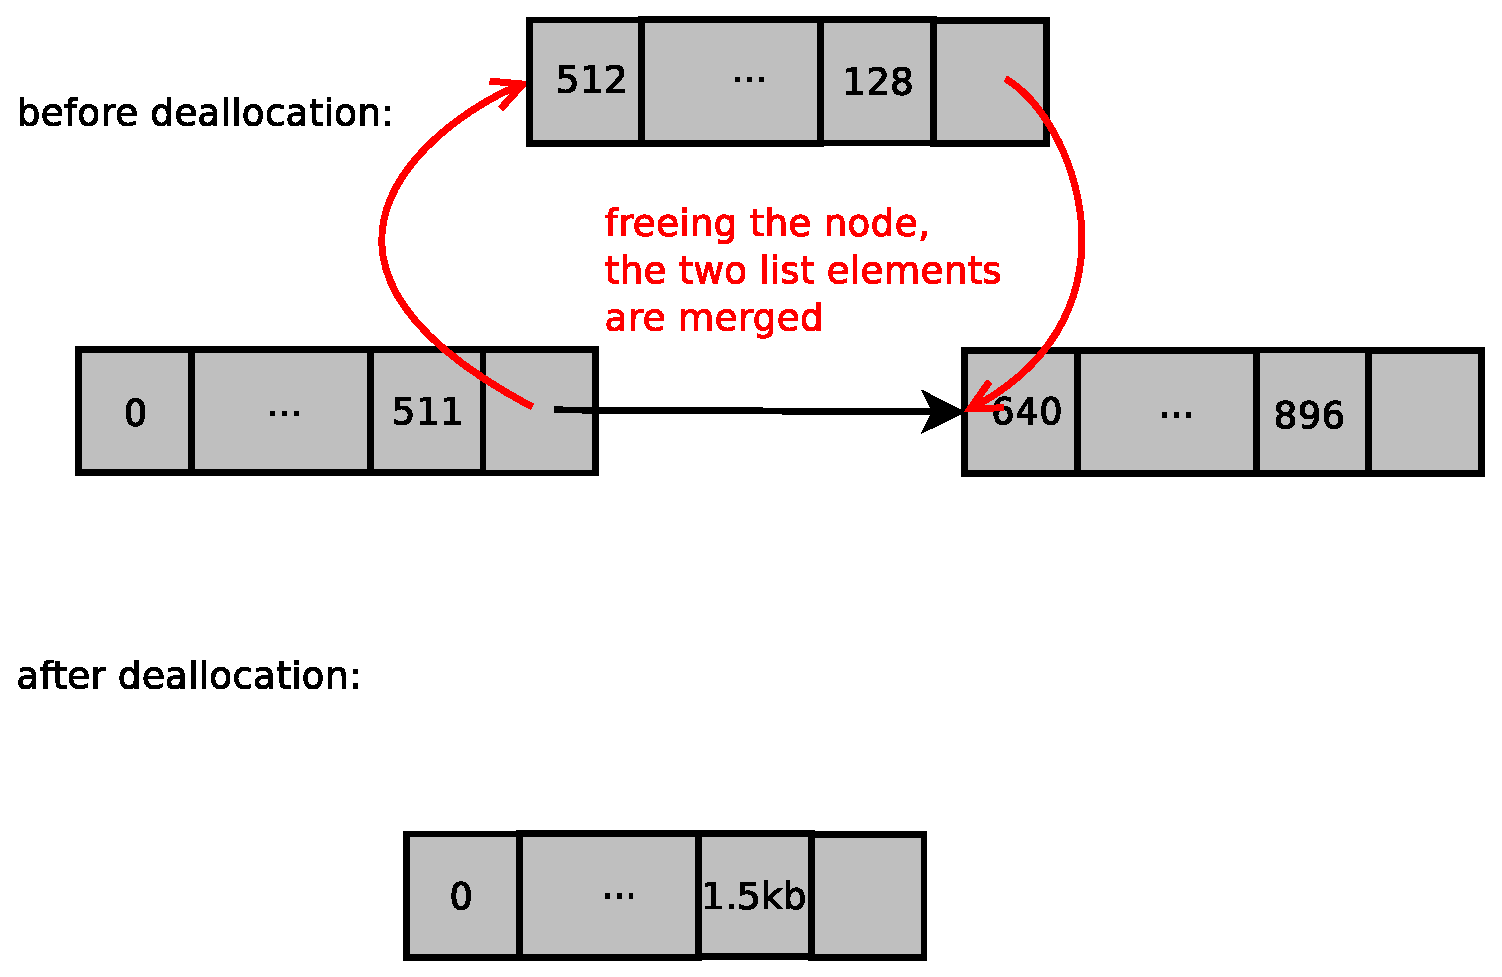
\includegraphics[width=0.7\columnwidth]{figures/free}
\caption{By freeing data at base pointer 512, creates a continueous space between base pointer 0 and
base pointer 640, causing the list nodes to merge into one.}
\label{fig:free}
\end{figure}

As soon as a process retrieves a future value, it makes a local copy of it, and frees any shared address space
that is associated with the future.  In order to free shared space, a process needs to provide the Shared\_pointer
that was returned by the allocator routine.  The Shared\_pointer keeps information of the page size used to 
allocate space, thus finding the correct free list is trivial, we just need to use the page size as an index.
We then insert the Shared\_pointer in the free list in a sorted fashion, using the base address for comparison.
This way, all free lists are sorted lists of Shared\_pointers by base address, so that if we find continueous
space, we merge the list elements, resulting in larger block of free space.  Figure~\ref{fig:free} shows a 
free list, before and after freeing some shared memory.  Because freeing 128 bytes at base address 512 creates
a continueous space from byte 0 to byte 640, the two list nodes will be merged into one.

\section{Scheduler}
\label{sect:scheduler}
In order to have a distributed memory interface similar to the shared memory one, we chose to implement 
a scheduler, which is responsible for deciding who will execute which \emph{job}.  If the user was 
responsible for distributing \emph{jobs} among the processes,  he would need to reason about dependencies
between \emph{jobs} and retrieving future values, else the program could easily end up in a deadlock.
To make our case clear, consider the fibonacci example in figure~\ref{lst:fib}.  
In our example, let's say we have
3 processes, one of them is the master process.  We need to run fib(3), thus, process 0, the master process 
can issue async(f, 2) to process 1 and async(f, 1) to process 2.  Process 1 can issue async(f, 1) to 
process 2 and run async(f, 0) on itself.  In this scenario the program will execute correctly without any
problems, since when any of the processes call a get() will either retrieve or wait for the value.  But 
consider we want to compute fib(5).  Process 1 may have to run async(f, 4) while process 2 will have to run
async(f, 3).  At some point, process 1 issues async(f, 3) to process 2, while process 2 issues an async(f, 2)
to process 1.  Both processes will return from the async calls and proceed calling get() to retrieve the value
but will actually block forever, since neither process will run the pending fibonacci functions.  This scenario
is not a problem if processes are dynamically spawned, but if we have a static number of process, which is
common for mpi programs, we need to address such issues.  

\begin{figure}[here]
\center
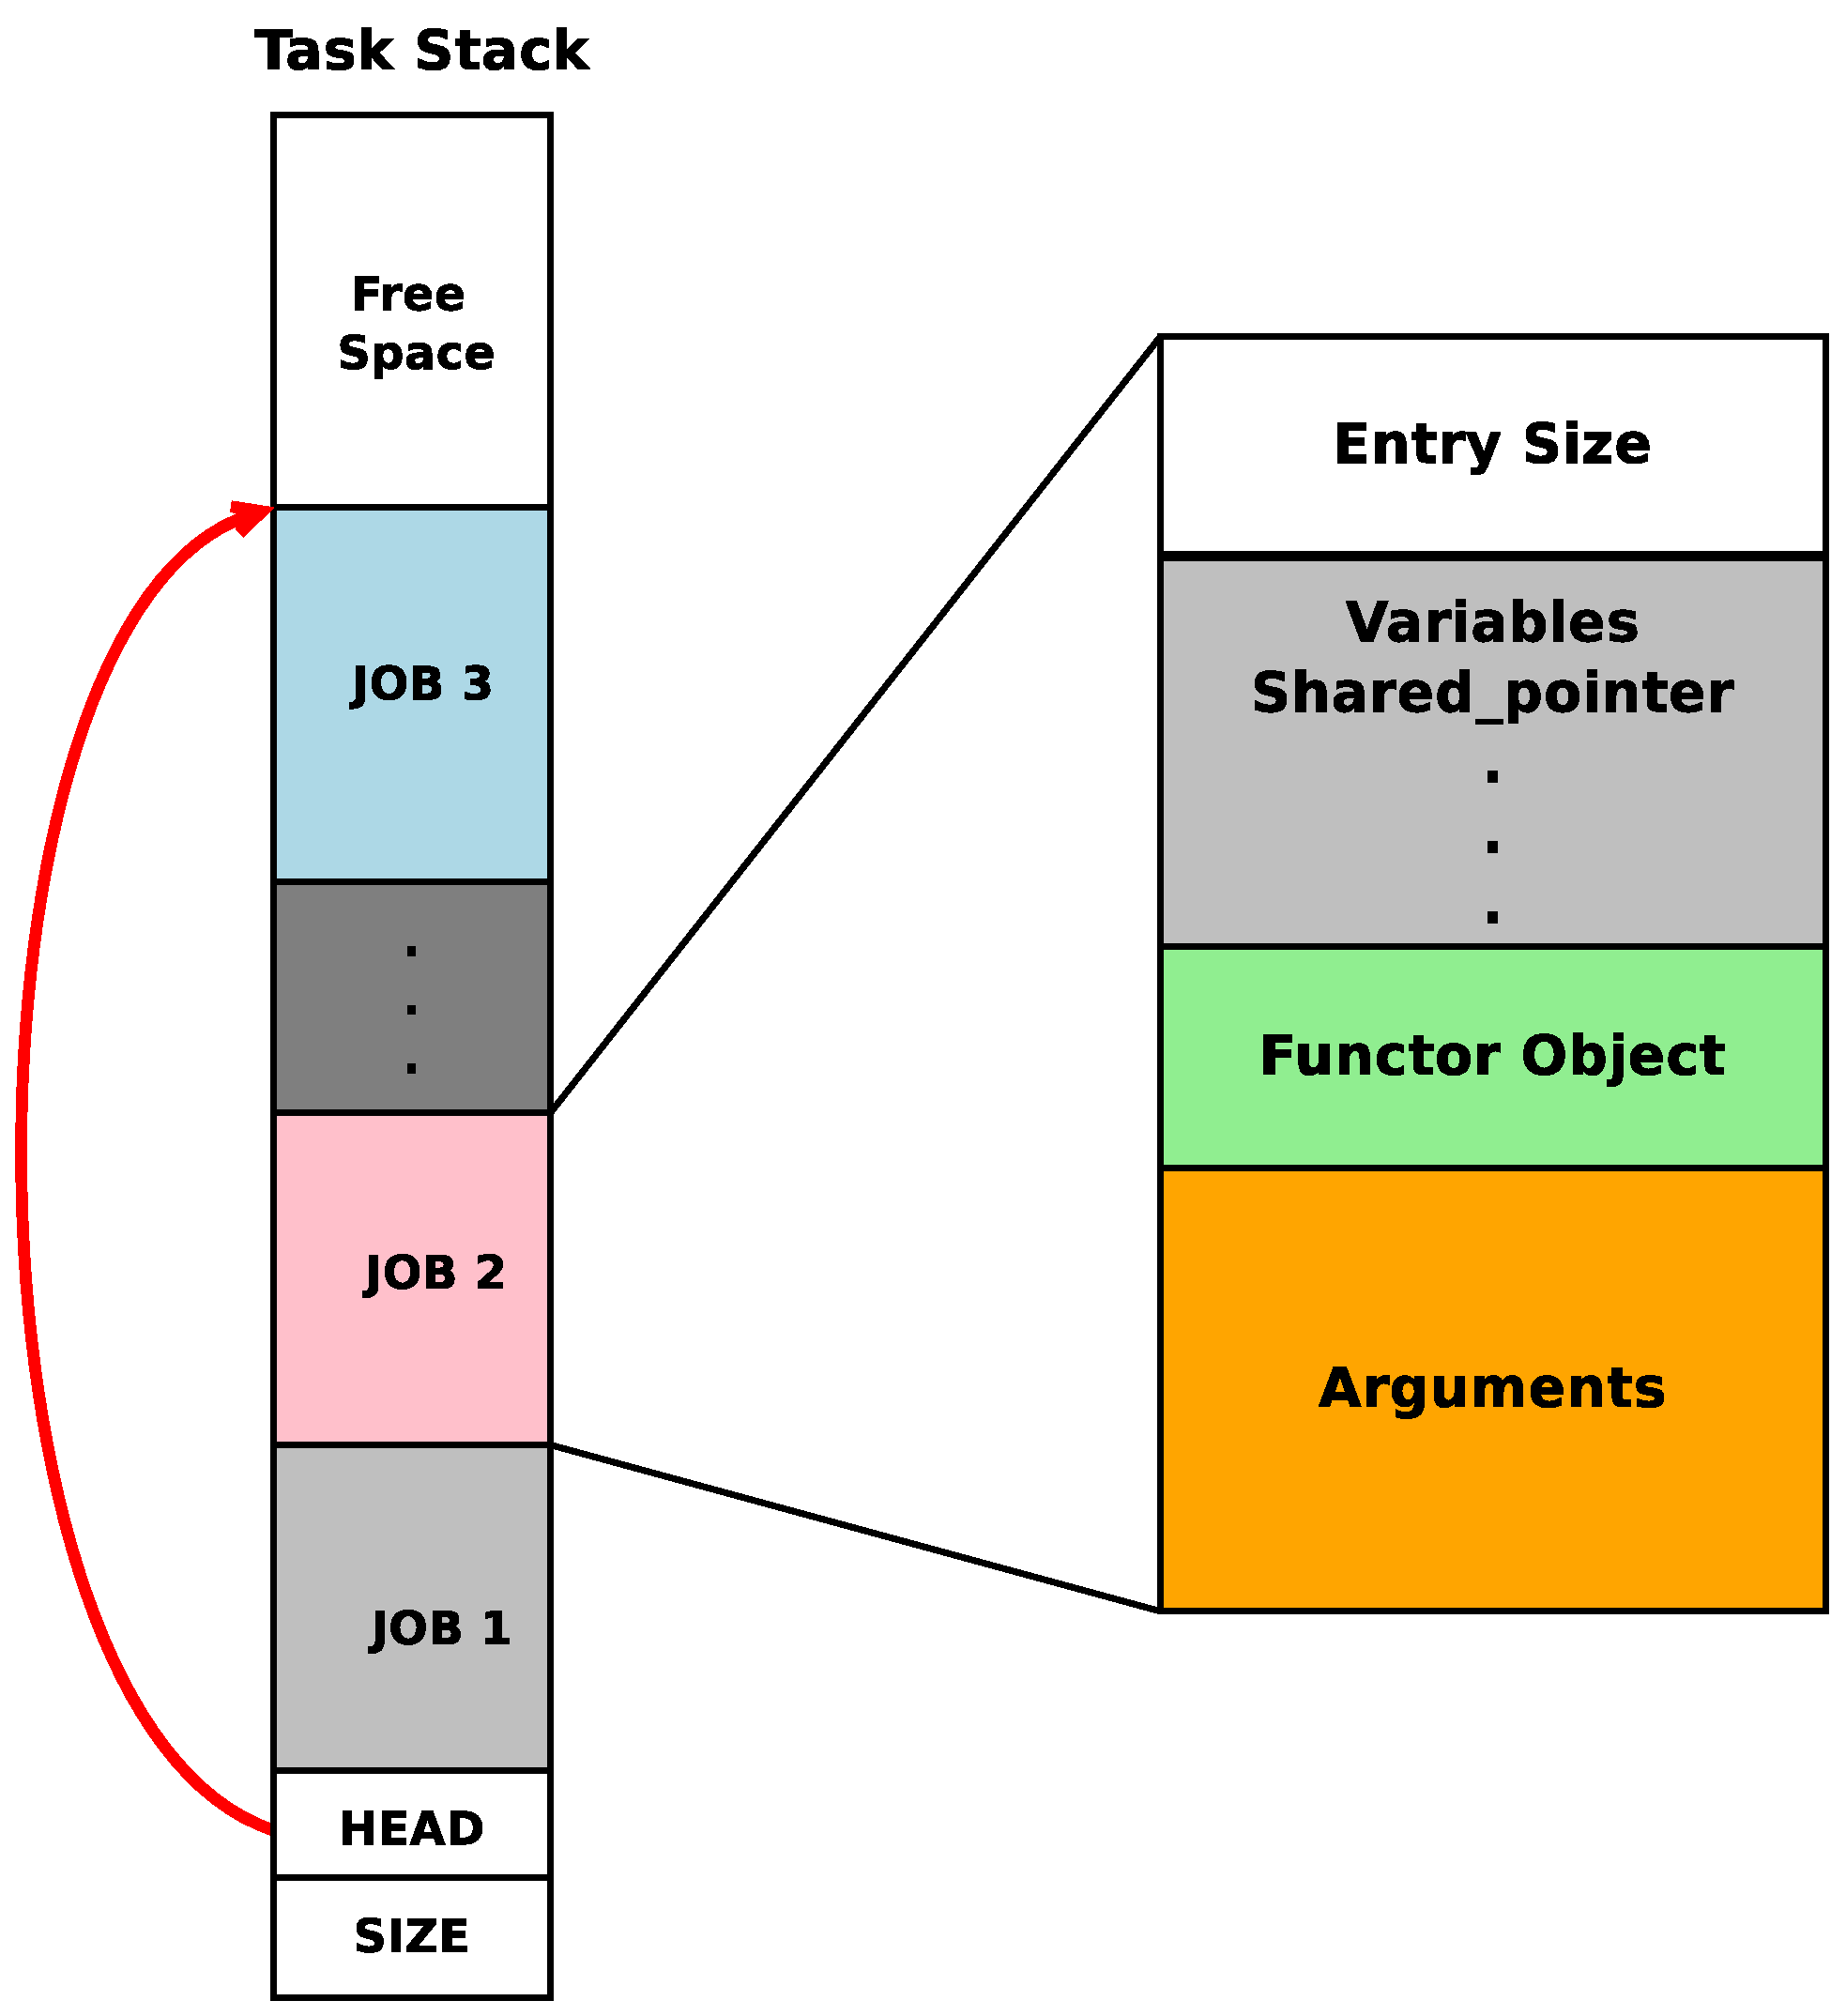
\includegraphics[width=0.5\columnwidth]{figures/task_stack}
\caption{Shared stack where a worker process keeps its pending jobs.  Entries can have varied sizes, this
size is stored at the beggining of the entry and can be used to retrieve the corresponding job.  Information
for the specific stack,like size and head, are stored at the beggining of the shared space, so that other
processes can access them.}
\label{fig:task_stack}
\end{figure}

Since it is not always trivial to reason about such dependencies, we have implemented our own \emph{job} 
scheduler.  We use MPI-2's one-sided communication library (via the communication module) to implement task
stacks, similar to their shared memory counterparts. We choose to implement a stack because it suits better
future logic, we need to execute the latest issued \emph{job} in order for the get() not to block indefinitely
in recursive algorithms.  Using one-sided communication, only the issuer needs to copy the functor object to
the workers stack, as in a shared memory environment.  Figure~\ref{fig:task_stack} 
shows how a task stack is structured.  
Note that an entry is composed by the functor object, its arguments (they are considered one object) and the 
size of the entry. This is neccessary since different functors and/or different arguments result in 
varying entry sizes.
Thus, the exact location of a \emph{job} is calculated using the stack head and functor object size values 
\footnote{functors and arguments are send/received as outpur/input archives, using boost.serialize library.}.
Moreover, at the beggining of the shared space, the size and current head values are stored, so all processes
can push \emph{jobs}.


Figure~\ref{fig:helloCF} shows a control flow graph for the master and worker processes.  
The master simply initializes
the futures environment and issues async functions while executing user code.  At the end it finalizes 
the futures environment and calls the terminate routine from the scheduler.  The workers initialize 
the futures environment, which must happen collectively among all workers and master and then enter a
loop, looking for pending jobs in their stacks until their terminate routine returns true, in which case
they exit the loop, finalize again collectively with all other processes and exit the program, without ever
returning to the main function.  The scheduler is responsible for providing the functionallity of the terminate
routines.  In our implementation the workers poll a local variable which they expose through the communication
module as a shared variable.  The master, when calling his terminate routine, will check the status of every 
worker.  A process can be either idle, busy or terminated.  Process status is again exposed by a shared variable
on each process.  The master will check the status of all the processes and if all of them are in idle status, he
will set the terminated flag to true on all of them.  If a process is still busy, meaning executes some \emph{job}
or has still pending \emph{jobs} in its stack, the master must wait till all jobs are finished and then set the 
terminated flags.

When running user code or a \emph{job} and an async call is made, the process will address the scheduler in order
to get the id of the next avaible process and allocates enough space for the return value to be stored.
Then it asks the scheduler to send the job to the worker process.  In our implementation the scheduler 
pushes the job int the process' stack.  Our scheduler distributes \emph{jobs} in a round robin fashion 
(excluding the master process, which should run user code). 

\subsection{Alternative Implementations/Design Versability}

We have designed the system to be able to use alternative scheduler implementations.  However, all must meet the
following interface requirments.\\

\begin{itemize}

 \item Implement routines to send and receive jobs.  The call to the \emph{async} function should be
able to send a \emph{job} to the worker process without blocking.  The worker should be able to handle
multiple \emph{jobs}, without breaking the asynchrous model.  Moreover, \emph{communication} should only
require the process that issued the \emph{job} and the one that receives it to participate.


 \item Implement a routine which returns a valid process id that is available to run a \emph{job}
issued by call to \emph{async}.

 \item Implement the terminate routine, which should return true for a process to exit and should
also not block execution if it does not return true.

\end{itemize}
 
\vfill

Remote Procedure Call (RMC) and Remote Method Invocation (RMI) libraries often have the above requirements as well.
There is a number of known solutions as to how to implement such systems in the literature.  The two most commonly used methods are polling for work requests
~\cite{Beckman96tulip:a, Saunders:2003:AAP:966049.781534, Foster96thenexus, vonEicken:1992:AMM:146628.140382} 
and hardware interrupts.
In our system, polling would require a worker process to poll for incoming \emph{jobs} at certain
time intervals.   Extra care must be taken to define the polling period, since if polling happens too often, it can
dominate computation, but we also need a process to poll frequent enough to ensure timely responses
~\cite{Saunders:2003:AAP:966049.781534, Shah:1998:PEL:876880.879642}.
Alternatively, a hardware interrupt could be sent to notify a process of an incoming message.  This method however,
is avoided because interrupts have to go through the OS, which has a significant cost. 
~\cite{Saunders:2003:AAP:966049.781534, Shah:1998:PEL:876880.879642, Foster96thenexus, vonEicken:1992:AMM:146628.140382}.
The Nexus system ~\cite{Foster96thenexus}, also suggests 

